The functions deployed in Serverless run on-demand and webmasters are billed by the millisecond of execution time. Therefore, if the function is unused, it's \textit{free}. In this case, everything that the application needs to run is completely abstracted by the cloud platform, and in turn, it handles failover, scalability, load balancing, etc. Like other architectures, the server-side logic is still written by the application developers but in contrast, the logic here is in the form of individual functions that are run in event-triggered and ephemeral stateless compute containers and are managed by a third party completely. The containers are created on demand and destroyed as soon as the function is executed. These functionalities have catered to Serverless architecture gaining huge popularity over time (Figure~\ref{fig:ServerlessPopularity})\footnote{Google Trends, “Popularity of the keyword Serverless,” 2019. http://bit.ly/GoogleServerless}. Amazon's AWS Lambda \footnote{Amazon, “AWS Lambda – Serverless Compute - Amazon Web Services.” https://aws.amazon.com/lambda/} is currently the most popular provider of Serverless Architectures. However, other players like Google Cloud Functions \footnote{Google, “Cloud Functions - Event-driven Serverless Computing.”
	https://cloud.google.com/functions/}, Azure Functions \footnote{Microsoft, “Azure Functions—Serverless Architecture.” https://azure.microsoft.com/en-us/services/functions/}, IMB Cloud Functions \footnote{IBM, “IBM Cloud Functions.” https://console.bluemix.net/openwhisk/} and Pivotal Function Service \footnote{Pivotal Software, “Pivotal Function Service (PFS),” jan 2017.
	https://pivotal.io/platform/pivotal-function-service} have also started gaining popularity.

\begin{figure}[h]
	\begin{framed}
		\centering
		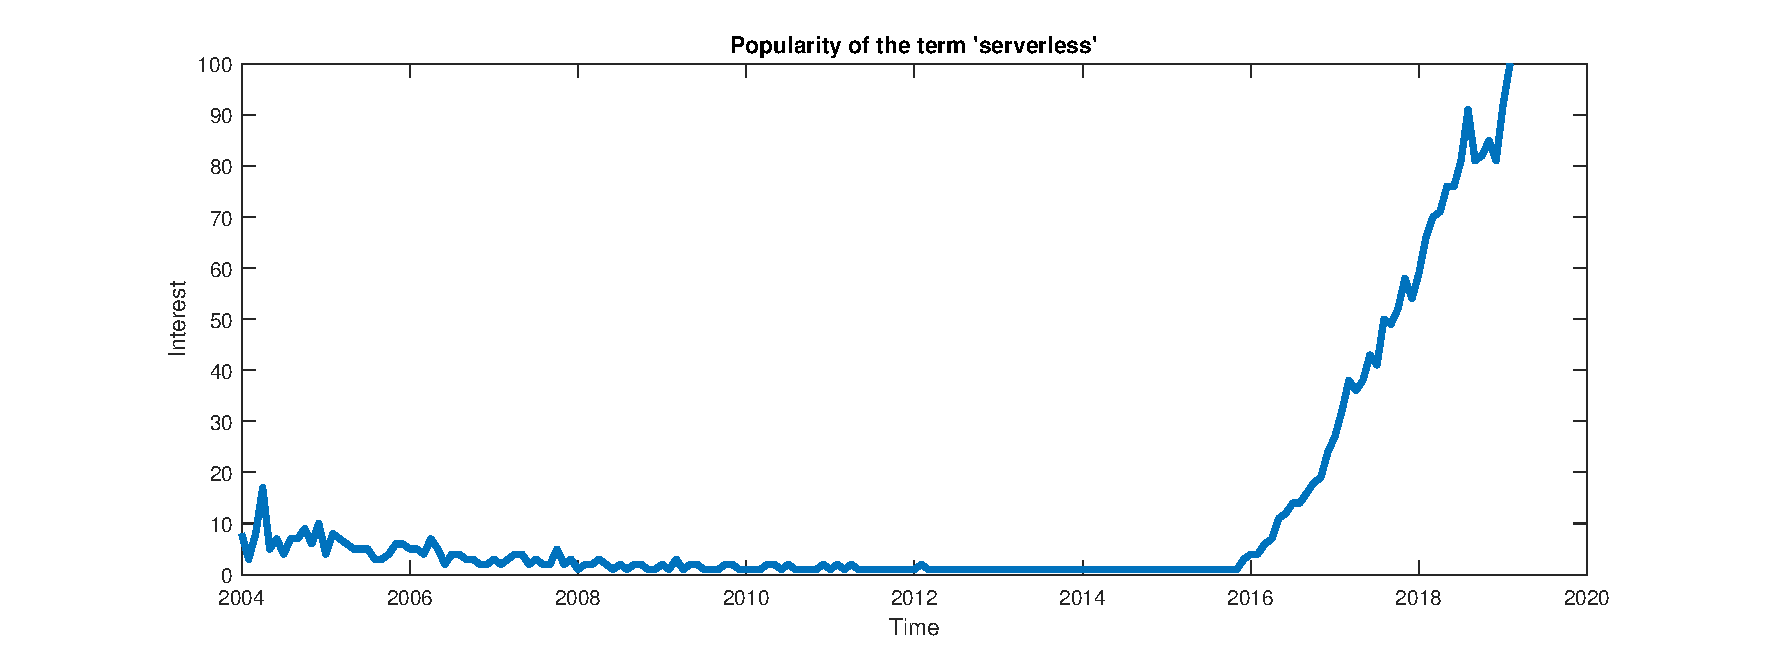
\includegraphics[width=\textwidth, trim={2.45cm 0 2.45cm 0},clip]{images/serverless_popularity.eps}
		\caption{A trends graph from Google showing the search interest of the term \textit{serverless} over the past fifteen years. Numbers represent search interest relative to the highest point on the chart for the given region and time. A value of 100 is the peak popularity for the term. A value of 50 means that the term is half as popular.}
		\label{fig:ServerlessPopularity}
		
	\end{framed}
\end{figure}

With the benefit of pay-per-use, zero-administration, ease of deployment and auto-scaling, Serverless also comes with new vulnerabilities. It does not have adequate security testing, as testing a serverless application can be far more complex than standard applications. As a result, many scanning tools haven't yet adapted to Serverless applications. Secondly, the application has an increased attack surface, as it consumes data from many event sources, namely cloud storage, HTTP APIs, IoT device communications, message queues, etc. A report from Puresec \cite{Segal2018} describes in detail the ten most critical security risks in Serverless architectures. Hence, a robust solution for the security of Serverless applications is needed.